%%%%%%%%%%%%%%%%%%%%%%%%%%%%%%%%%%%%%%%%%%
%%%%%%%%%%%%%                 %%%%%%%%%%%%
%%%%%%%%%%%%%    EXERCISE 1   %%%%%%%%%%%%
%%%%%%%%%%%%%                 %%%%%%%%%%%%
%%%%%%%%%%%%%%%%%%%%%%%%%%%%%%%%%%%%%%%%%%
\begin{exercise}[]{Consider a datagram network using 32-bit host addresses. Suppose a router has four links, numbered 0 through 3, and packets are to be forwarded to the link interfaces as follows: (20 points)
    \begin{figure}[hb]
      \begin{center}
      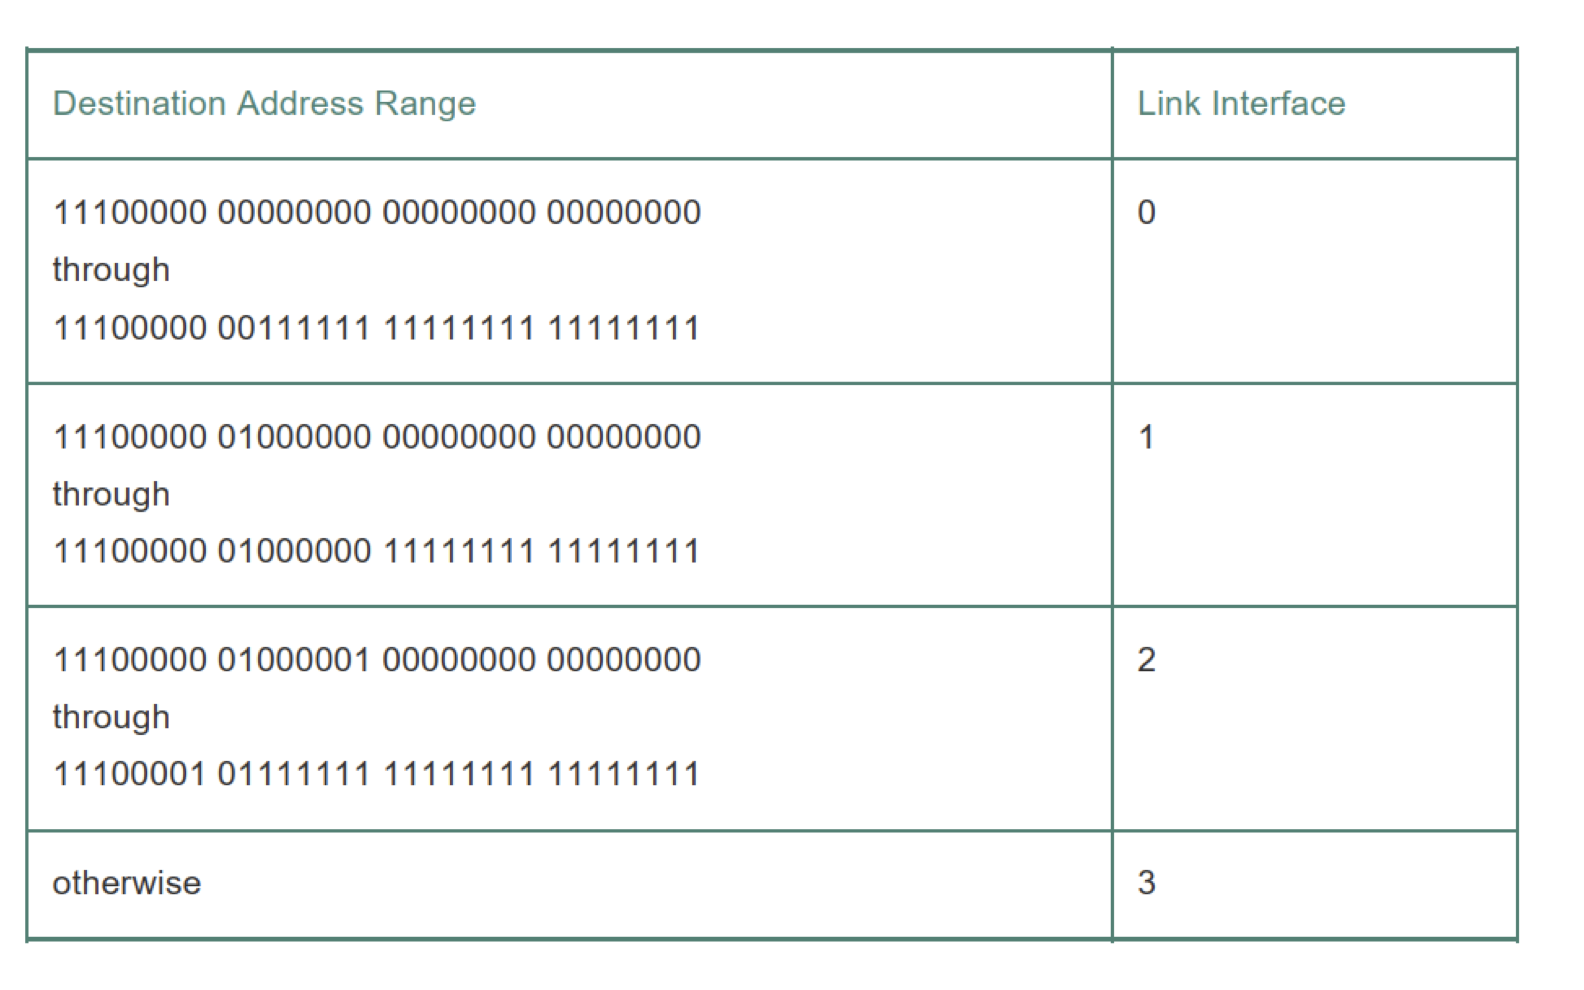
\includegraphics[width=12cm]{img/ass4/ex1}
      \caption{Exercise 1}
      \label{fig:ex1}
      \end{center}
    \end{figure}
    \begin{enumerate}
        \item Provide a forwarding table that has four entries, uses longest prefix matching, and forwards packets to the correct link interfaces. (5 points)
        \item Rewrite this forwarding table using the a.b.c.d/x notation instead of the binary string notation. (5 points)
        \item Describe how your forwarding table determines the appropriate link interface for data- grams with destination addresses: (10 points)
        \begin{verbatim}
            11001000 10010001 01010001 01010101
            11100001 01000000 11000011 00111100
            11100001 10000000 00010001 01110111
        \end{verbatim}
    \end{enumerate}
    }
  \begin{solution}
  \par{~}
  \begin{enumerate}
    \item The forwarding table is presented in Table \ref{tab:ex1-1}.
    \begin{table}[h]
      \centering
      \begin{tabular}{lc}
      \hline
      \multicolumn{1}{c}{\textbf{Prefix}} & \textbf{Link Interface} \\ \hline
      11100000                            & 0                       \\
      11100000 01000000                   & 1                       \\
      1110000                             & 2                       \\
      11100001 1                          & 3                       \\
      otherwise                           & 3                       \\ \hline
      \end{tabular}
      \caption{Forwarding Table \label{tab:ex1-1}}
    \end{table}
    \item The forwarding table is presented in Table \ref{tab:ex1-2}.
    \begin{table}[h]
      \centering
      \begin{tabular}{lc}
      \hline
      \multicolumn{1}{c}{\textbf{Prefix}} & \textbf{Link Interface} \\ \hline
      224.0.0.0/8                            & 0                       \\
      224.64.0.0/16                  & 1                       \\
      224.0.0.0/7                     & 2                       \\
      224.128.0.0/9                          & 3                       \\
      otherwise                           & 3                       \\ \hline
      \end{tabular}
      \caption{Forwarding Table \label{tab:ex1-2}}
    \end{table}
    \item \begin{enumerate}
      \item \texttt{11001000 10010001 01010001 01010101} matches the last entry. Link interface is 3.
      \item \texttt{11100001 01000000 11000011 00111100} matches the third entry. Link interface is 2.
      \item \texttt{11100001 10000000 00010001 01110111} matches the  fourth entry. Link interface is 3.
    \end{enumerate}
  \end{enumerate}
  \end{solution}
  \label{ex1}
\end{exercise}




%%%%%%%%%%%%%%%%%%%%%%%%%%%%%%%%%%%%%%%%%%
%%%%%%%%%%%%%                 %%%%%%%%%%%%
%%%%%%%%%%%%%    EXERCISE 2   %%%%%%%%%%%%
%%%%%%%%%%%%%                 %%%%%%%%%%%%
%%%%%%%%%%%%%%%%%%%%%%%%%%%%%%%%%%%%%%%%%%
\begin{exercise}[]{Consider the topology shown below. (20 points)
  \begin{enumerate}
    \item Assign network addresses to each of these six subnets, with the following constraints:
    All addresses must be allocated from 214.97.254/23; Subnet A should have enough  addresses to support 250 interfaces; Subnet B should have enough addresses to support
    120 interfaces; and Subnet C should have enough addresses to support 120 interfaces.
    Of course, subnets D, E and F should each be able to support two interfaces. For each
    subnet, the assignment should take the form a.b .c.d/x or a. b. c .d/x – e. f. g. h/y.
    (10 points)
    \item Using your answer to part 1, provide the forwarding tables (using longest prefix matching) for each of the three routers. (10 points)
  \end{enumerate}}
  \begin{figure}[hb]
    \begin{center}
    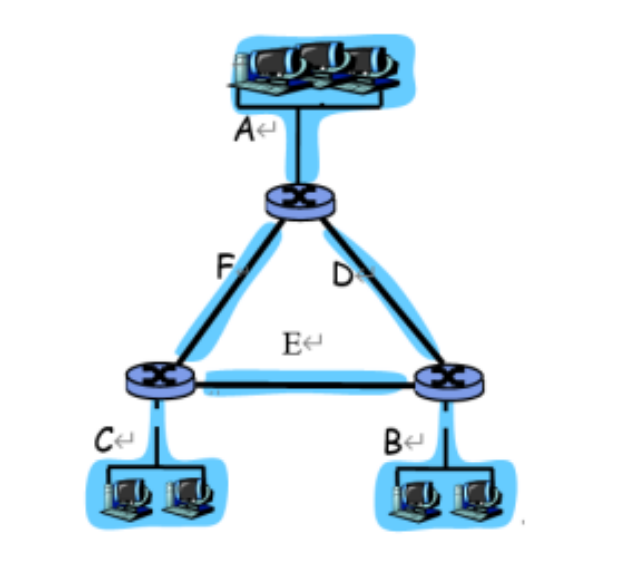
\includegraphics[width=6cm]{img/ass4/ex2}
    \caption{The topology in P2}
    \label{fig:ex2}
    \end{center}
  \end{figure}
  \begin{solution}
  \par{~}
  \begin{enumerate}
    \item The assignment is listed in Table \ref{tab:ex2}
    \begin{table}[h]
      \centering
      \begin{tabular}{lc}
      \hline
      \multicolumn{1}{c}{\textbf{Assignment}} & \textbf{Link Interface} \\ \hline
      214.97.254.0/24      & A                       \\
      214.97.255.0/25                  & B                       \\
      214.97.255.128/25 - 214.97.255.248/29 & C                       \\
      214.97.255.248/31  & D                      \\
      214.97.255.250/31  & E                      \\
      214.97.255.252/31  & F                      \\\hline
      \end{tabular}
      \caption{Forwarding Table \label{tab:ex2}}
    \end{table}
    \item The forwarding tables are listed in Table \ref{tab:ex2-2}, \ref{tab:ex2-3}, \ref{tab:ex2-4}.
    \begin{table}[h]
      \centering
      \begin{tabular}{lc}
      \hline
      \multicolumn{1}{c}{\textbf{Prefix}} & \textbf{Link Interface} \\ \hline
      11010110 01100001 11111110      & A                       \\
      11010110 01100001 11111111 0    & B                       \\
      11010110 01100001 11111111 1111100 & B                      \\
      11010110 01100001 11111111 1 &C                      \\\hline
      \end{tabular}
      \caption{Forwarding Table for top router \label{tab:ex2-2}}
    \end{table}

    \begin{table}[h]
      \centering
      \begin{tabular}{lc}
      \hline
      \multicolumn{1}{c}{\textbf{Prefix}} & \textbf{Link Interface} \\ \hline
      11010110 01100001 11111110      & F                       \\
      11010110 01100001 11111111 1111110 & F                      \\
      11010110 01100001 11111111 111110 & E                      \\
      11010110 01100001 11111111 0    & E                       \\
      11010110 01100001 11111111 1 &C                      \\\hline
      \end{tabular}
      \caption{Forwarding Table for bottom-left router \label{tab:ex2-3}}
    \end{table}

    \begin{table}[h]
      \centering
      \begin{tabular}{lc}
      \hline
      \multicolumn{1}{c}{\textbf{Prefix}} & \textbf{Link Interface} \\ \hline
      11010110 01100001 11111111 0    & B                       \\
      11010110 01100001 11111110      & D                       \\
      11010110 01100001 11111111 1111100 & D                      \\
      11010110 01100001 11111111 1 &E                      \\\hline
      \end{tabular}
      \caption{Forwarding Table for bottom-right router \label{tab:ex2-4}}
    \end{table}
  \end{enumerate}
  \end{solution}
  \label{ex2}
\end{exercise}


%%%%%%%%%%%%%%%%%%%%%%%%%%%%%%%%%%%%%%%%%%
%%%%%%%%%%%%%                 %%%%%%%%%%%%
%%%%%%%%%%%%%    EXERCISE 3   %%%%%%%%%%%%
%%%%%%%%%%%%%                 %%%%%%%%%%%%
%%%%%%%%%%%%%%%%%%%%%%%%%%%%%%%%%%%%%%%%%%
\begin{exercise}[]{Consider the network shown below, and assume that each node initially knows
  the costs to each of its neighbors. Consider the distance-vector algorithm and show the
  distance table entries at node z. (20 points)}

  \begin{figure}[hb]
    \begin{center}
    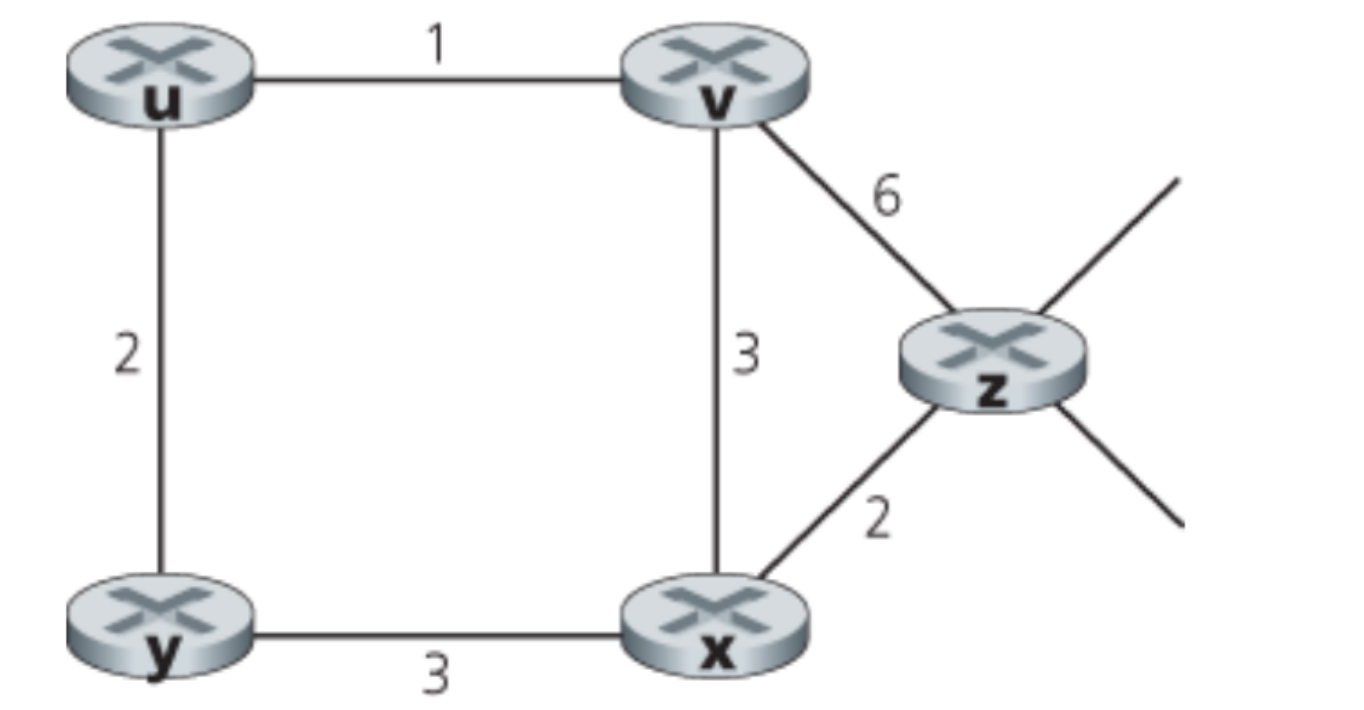
\includegraphics[width=6cm]{img/ass4/ex3}
    \caption{The network in P3}
    \label{fig:ex3}
    \end{center}
  \end{figure}
  \begin{solution}
  \par{~}
  See Table \ref{tab:ex3}

  \begin{table}[h]
    \centering
    \begin{tabular}{llllll}\hline
    initial & u & v & x & y & z \\
    v                & $\infty$          & $\infty$ & $\infty$ & $\infty$ & $\infty$ \\
    x                & $\infty$          & $\infty$ & $\infty$ & $\infty$ & $\infty$ \\
    z                & $\infty$          & 6 & 2 & $\infty$ & 0 \\\hline
    iter1            & u          & v & x & y & z \\
    v                & 1          & 0 & 3 & $\infty$ & 6 \\
    x                & $\infty$          & 3 & 0 & 3 & 2 \\
    z                & 7          & 5 & 2 & 5 & 0 \\\hline
    iter2            & u          & v & x & y & z \\
    v                & 1          & 0 & 3 & 3 & 5 \\
    x                & 4          & 3 & 0 & 3 & 2 \\
    z                & 6          & 5 & 2 & 5 & 0\\\hline
    \end{tabular}
    \caption{Distance Table \label{tab:ex3}}
    \end{table}
  \end{solution}
  \label{ex3}
\end{exercise}



%%%%%%%%%%%%%%%%%%%%%%%%%%%%%%%%%%%%%%%%%%
%%%%%%%%%%%%%                 %%%%%%%%%%%%
%%%%%%%%%%%%%    EXERCISE 4   %%%%%%%%%%%%
%%%%%%%%%%%%%                 %%%%%%%%%%%%
%%%%%%%%%%%%%%%%%%%%%%%%%%%%%%%%%%%%%%%%%%
\begin{exercise}[]{Please compare LSR and DVR, and explain each suitable usage scenarios. How
  Internet routing protocols deal with DVR count-to-infinity problem? (15 points)}
  \begin{solution}
  \par{~} Comparison between LSR and DVR are summarized as follows.
  \paragraph{Message complexity} Since LSR requies knowledge of the whole network, with $n$ nodes, $E$ links, it takes $O(nE)$ messages to be sent, while for DVR, only messages between connected nodes are required.
  \paragraph{Convergence speed} LSR can converge in $O(N\log N)$ time for every node, while the convergence for DVR is slower and is vulnerable to count-to-infinity problem.
  \paragraph{Robustness} Both LSR and DVR may broadcast incorrect link/path cost. In LSR, each node computes its own table, but in DVR, the error information can be propagated to the whole network.

  \par{~}

  One solution for count-to-infinity problem is \emph{poisoned reverse}. For example, if node Z  has decided to route through Y to get to X: 
  Z will tell Y its (Z’s) distance to X is infinite,  so that Y won’t route to X via Z. Poisoned reverse will partially resolve the count-to-infinity problem.
  \end{solution}
  \label{ex4}
\end{exercise}


%%%%%%%%%%%%%%%%%%%%%%%%%%%%%%%%%%%%%%%%%%
%%%%%%%%%%%%%                 %%%%%%%%%%%%
%%%%%%%%%%%%%    EXERCISE 5   %%%%%%%%%%%%
%%%%%%%%%%%%%                 %%%%%%%%%%%%
%%%%%%%%%%%%%%%%%%%%%%%%%%%%%%%%%%%%%%%%%%
\begin{exercise}[]{What’s the difference between Intra-AS Routing and Inter-AS Routing? (15
  points)}
  \begin{solution}
  \par{~}

  As for Intra-AS routing, the routing takes place among hosts, and the algorithm only involves routers in same AS. All routers in AS must run same intra-domain protocol. Intra-domain routing protocols (e.g. OSPF) ignores the internet outside the AS.
  
  As for Inter-AS routing, routing algorithm works within and between AS. The routers in different AS can run different intra-domain routing protocol. Inter-domain routing protocol (e.g. GBP) assumes that the internet contains the collection of interconnected AS.


  \end{solution}
  \label{ex5}
\end{exercise}


%%%%%%%%%%%%%%%%%%%%%%%%%%%%%%%%%%%%%%%%%%
%%%%%%%%%%%%%                 %%%%%%%%%%%%
%%%%%%%%%%%%%    EXERCISE 6   %%%%%%%%%%%%
%%%%%%%%%%%%%                 %%%%%%%%%%%%
%%%%%%%%%%%%%%%%%%%%%%%%%%%%%%%%%%%%%%%%%%
\begin{exercise}[]{Please explain methods to reduce the size of routing table. (15 points)}
  \begin{solution}
  \par{~}
  Hierarchical Routing is the main idea of reducing size of routing table as the number of routers in the network becomes large. To be specific, routers are organized into autonomous systems (ASs), with each AS consisting of a group of routers that are typically under the same administrative control (e.g., operated by the same ISP or belonging to the same company network). The routing running within an autonomous system are handled by intra-autonomous routing algorithms, while the routing among ASs are handled by inter-autonomous routing algorithms. Furthermore, modern intra-routing algorithms (e.g. Hierarchical OSPF) allow dividing the autonomous domain again into sub domains, so that internal routers only need to store the table with a limited size and that only a few "backbone routers" will need to store the whole information required by intra-autonomous routing. Therefore, the overall size of routing table in the network can be limited to a reasonable scale.
  \end{solution}
  \label{ex6}
\end{exercise}

%%%%%%%%%%%%%%%%%%%%%%%%%%%%%%%%%%%%%%%%%%
%%%%%%%%%%%%%                 %%%%%%%%%%%%
%%%%%%%%%%%%%    EXERCISE 7   %%%%%%%%%%%%
%%%%%%%%%%%%%                 %%%%%%%%%%%%
%%%%%%%%%%%%%%%%%%%%%%%%%%%%%%%%%%%%%%%%%%
\begin{exercise}[]{Please explain why we need IPv6 to replace IPv4. (15 points)}
  \begin{solution}
  \par{~} 
  The prime motivation for IPv6 was the realization that the 32-bit IP address space was beginning to be used up, with new subnets and IP nodes being attached to the Internet (and being allocated unique IP addresses) at a breathtaking rate. To respond to this need for a large IP address space, a new IP protocol, IPv6, was developed. In addition, IPv6 is also designed with the expectation that other aspects of IPv4 could be tweaked and augmented (e.g. flow labeling and priority), based on the accumulated operational experience with IPv4.
  \end{solution}
  \label{ex7}
\end{exercise}


%%%%%%%%%%%%%%%%%%%%%%%%%%%%%%%%%%%%%%%%%%
%%%%%%%%%%%%%                 %%%%%%%%%%%%
%%%%%%%%%%%%%    EXERCISE 8   %%%%%%%%%%%%
%%%%%%%%%%%%%                 %%%%%%%%%%%%
%%%%%%%%%%%%%%%%%%%%%%%%%%%%%%%%%%%%%%%%%%
\begin{exercise}[]{Company A needs 1024 IP addresses from an ISP who owns network prefix
  206.0.64.0/18. (30 points)

  Company A has 4 departments: Department1 requires 510 addresses which is further
  divided into 4 LANs(LAN1 LAN4); Department2 requires 256 addresses which is further
  divided into 4 LANs(LAN5 LAN8); Department3 requires 128 addresses which is further
  divided into 2 LANs(LAN9 LAN10); Department4 requires 128 addresses which is further
  divided into 2 LANs(LAN11 LAN12) . Another subnet LAN0 only needs 1 public IP address
  which uses NAT. please assign IP prefix to these 13 subnets with CIDR (Classless InterDomain Routing) technology. Please fill in the routing tables for RA, R1 and R3. Please
  aggregate entries if possible}
  \begin{solution}
  \par{~} See Figure \ref{fig:ex8}

  \begin{figure}[hb]
    \begin{center}
    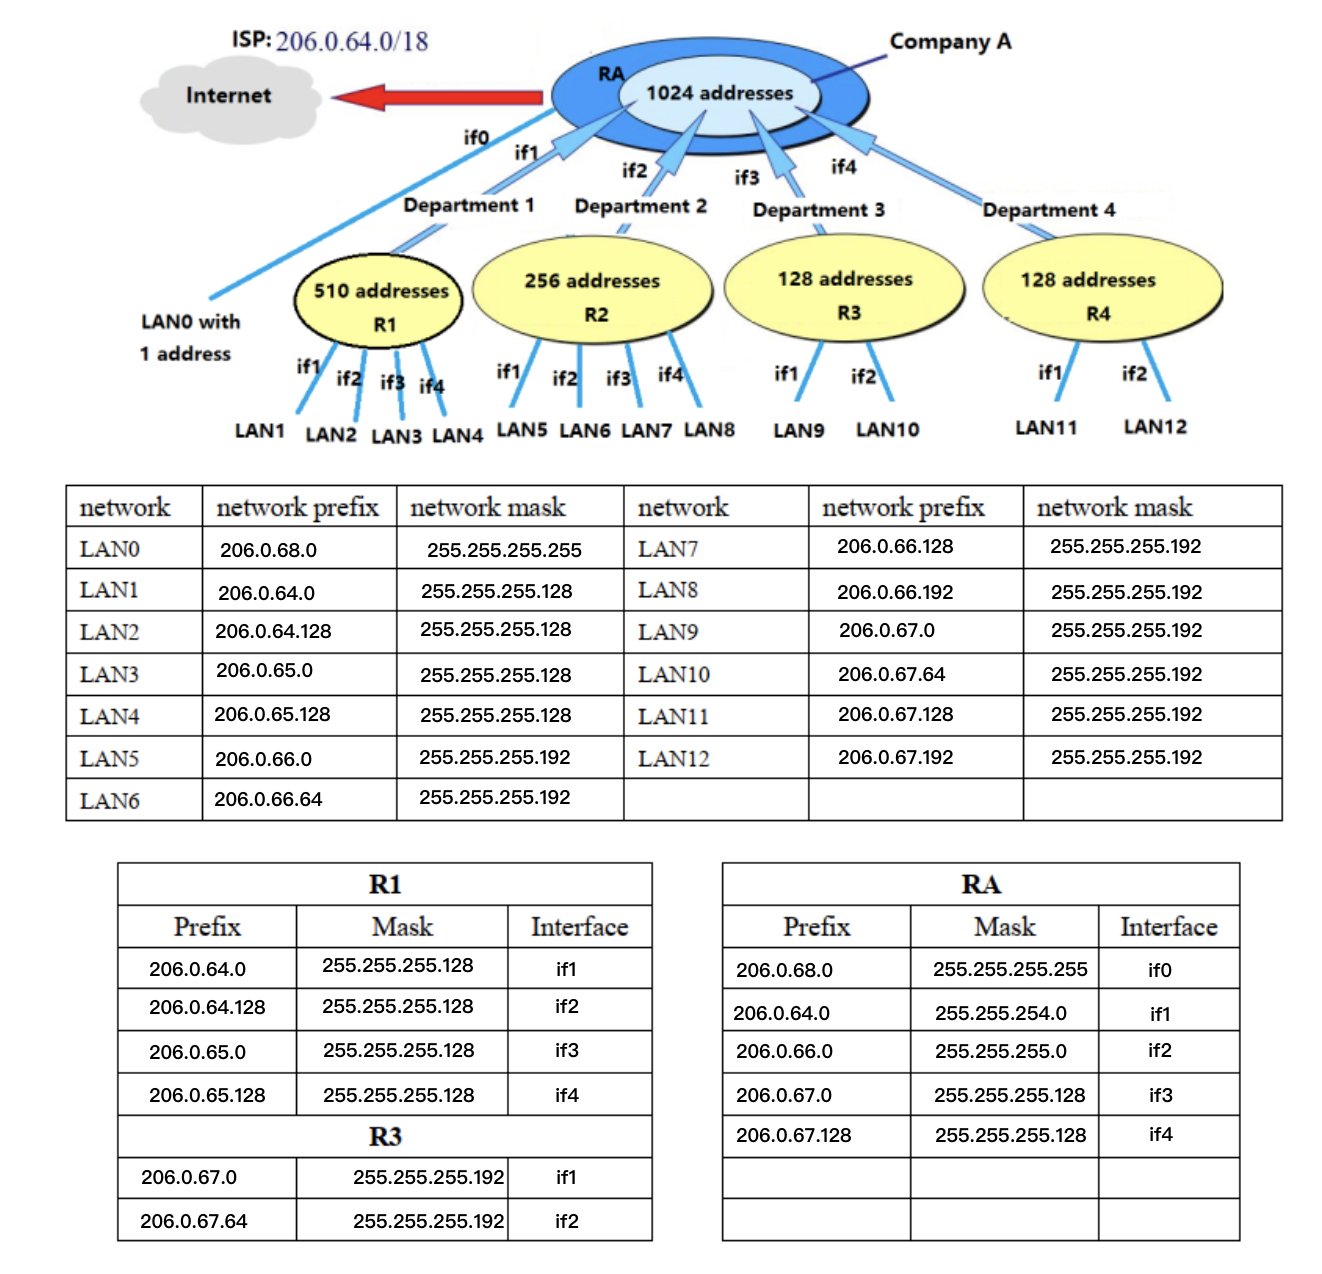
\includegraphics[width=12cm]{img/ass4/ex8}
    \caption{Exercise 8 solution}
    \label{fig:ex8}
    \end{center}
  \end{figure}
  \end{solution}
  \label{ex8}
\end{exercise}